% Created by tikzDevice version 0.12.6 on 2024-04-10 20:49:10
% !TEX encoding = UTF-8 Unicode
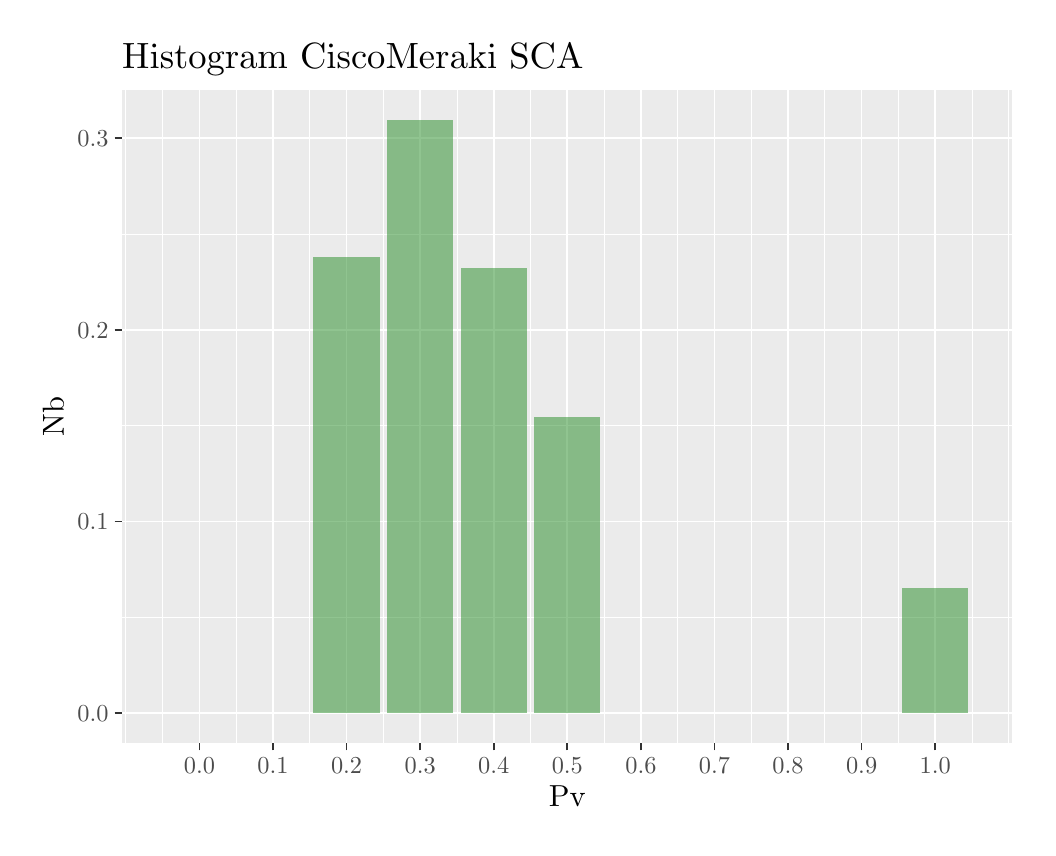
\begin{tikzpicture}[x=1pt,y=1pt]
\definecolor{fillColor}{RGB}{255,255,255}
\path[use as bounding box,fill=fillColor,fill opacity=0.00] (0,0) rectangle (361.35,289.08);
\begin{scope}
\path[clip] (  0.00,  0.00) rectangle (361.35,289.08);
\definecolor{drawColor}{RGB}{255,255,255}
\definecolor{fillColor}{RGB}{255,255,255}

\path[draw=drawColor,line width= 0.6pt,line join=round,line cap=round,fill=fillColor] (  0.00,  0.00) rectangle (361.35,289.08);
\end{scope}
\begin{scope}
\path[clip] ( 34.16, 30.69) rectangle (355.85,266.42);
\definecolor{fillColor}{gray}{0.92}

\path[fill=fillColor] ( 34.16, 30.69) rectangle (355.85,266.42);
\definecolor{drawColor}{RGB}{255,255,255}

\path[draw=drawColor,line width= 0.3pt,line join=round] ( 34.16, 76.02) --
	(355.85, 76.02);

\path[draw=drawColor,line width= 0.3pt,line join=round] ( 34.16,145.26) --
	(355.85,145.26);

\path[draw=drawColor,line width= 0.3pt,line join=round] ( 34.16,214.49) --
	(355.85,214.49);

\path[draw=drawColor,line width= 0.3pt,line join=round] ( 35.49, 30.69) --
	( 35.49,266.42);

\path[draw=drawColor,line width= 0.3pt,line join=round] ( 48.78, 30.69) --
	( 48.78,266.42);

\path[draw=drawColor,line width= 0.3pt,line join=round] ( 75.36, 30.69) --
	( 75.36,266.42);

\path[draw=drawColor,line width= 0.3pt,line join=round] (101.95, 30.69) --
	(101.95,266.42);

\path[draw=drawColor,line width= 0.3pt,line join=round] (128.54, 30.69) --
	(128.54,266.42);

\path[draw=drawColor,line width= 0.3pt,line join=round] (155.12, 30.69) --
	(155.12,266.42);

\path[draw=drawColor,line width= 0.3pt,line join=round] (181.71, 30.69) --
	(181.71,266.42);

\path[draw=drawColor,line width= 0.3pt,line join=round] (208.30, 30.69) --
	(208.30,266.42);

\path[draw=drawColor,line width= 0.3pt,line join=round] (234.88, 30.69) --
	(234.88,266.42);

\path[draw=drawColor,line width= 0.3pt,line join=round] (261.47, 30.69) --
	(261.47,266.42);

\path[draw=drawColor,line width= 0.3pt,line join=round] (288.06, 30.69) --
	(288.06,266.42);

\path[draw=drawColor,line width= 0.3pt,line join=round] (314.64, 30.69) --
	(314.64,266.42);

\path[draw=drawColor,line width= 0.3pt,line join=round] (341.23, 30.69) --
	(341.23,266.42);

\path[draw=drawColor,line width= 0.3pt,line join=round] (354.52, 30.69) --
	(354.52,266.42);

\path[draw=drawColor,line width= 0.6pt,line join=round] ( 34.16, 41.40) --
	(355.85, 41.40);

\path[draw=drawColor,line width= 0.6pt,line join=round] ( 34.16,110.64) --
	(355.85,110.64);

\path[draw=drawColor,line width= 0.6pt,line join=round] ( 34.16,179.88) --
	(355.85,179.88);

\path[draw=drawColor,line width= 0.6pt,line join=round] ( 34.16,249.11) --
	(355.85,249.11);

\path[draw=drawColor,line width= 0.6pt,line join=round] ( 62.07, 30.69) --
	( 62.07,266.42);

\path[draw=drawColor,line width= 0.6pt,line join=round] ( 88.66, 30.69) --
	( 88.66,266.42);

\path[draw=drawColor,line width= 0.6pt,line join=round] (115.24, 30.69) --
	(115.24,266.42);

\path[draw=drawColor,line width= 0.6pt,line join=round] (141.83, 30.69) --
	(141.83,266.42);

\path[draw=drawColor,line width= 0.6pt,line join=round] (168.42, 30.69) --
	(168.42,266.42);

\path[draw=drawColor,line width= 0.6pt,line join=round] (195.00, 30.69) --
	(195.00,266.42);

\path[draw=drawColor,line width= 0.6pt,line join=round] (221.59, 30.69) --
	(221.59,266.42);

\path[draw=drawColor,line width= 0.6pt,line join=round] (248.18, 30.69) --
	(248.18,266.42);

\path[draw=drawColor,line width= 0.6pt,line join=round] (274.76, 30.69) --
	(274.76,266.42);

\path[draw=drawColor,line width= 0.6pt,line join=round] (301.35, 30.69) --
	(301.35,266.42);

\path[draw=drawColor,line width= 0.6pt,line join=round] (327.93, 30.69) --
	(327.93,266.42);
\definecolor{fillColor}{RGB}{34,139,34}

\path[fill=fillColor,fill opacity=0.50] (103.28, 41.40) rectangle (127.21,206.25);

\path[fill=fillColor,fill opacity=0.50] (129.87, 41.40) rectangle (153.79,255.71);

\path[fill=fillColor,fill opacity=0.50] (156.45, 41.40) rectangle (180.38,202.13);

\path[fill=fillColor,fill opacity=0.50] (183.04, 41.40) rectangle (206.97,148.55);

\path[fill=fillColor,fill opacity=0.50] (315.97, 41.40) rectangle (339.90, 86.74);
\end{scope}
\begin{scope}
\path[clip] (  0.00,  0.00) rectangle (361.35,289.08);
\definecolor{drawColor}{gray}{0.30}

\node[text=drawColor,anchor=base east,inner sep=0pt, outer sep=0pt, scale=  0.88] at ( 29.21, 38.37) {0.0};

\node[text=drawColor,anchor=base east,inner sep=0pt, outer sep=0pt, scale=  0.88] at ( 29.21,107.61) {0.1};

\node[text=drawColor,anchor=base east,inner sep=0pt, outer sep=0pt, scale=  0.88] at ( 29.21,176.85) {0.2};

\node[text=drawColor,anchor=base east,inner sep=0pt, outer sep=0pt, scale=  0.88] at ( 29.21,246.08) {0.3};
\end{scope}
\begin{scope}
\path[clip] (  0.00,  0.00) rectangle (361.35,289.08);
\definecolor{drawColor}{gray}{0.20}

\path[draw=drawColor,line width= 0.6pt,line join=round] ( 31.41, 41.40) --
	( 34.16, 41.40);

\path[draw=drawColor,line width= 0.6pt,line join=round] ( 31.41,110.64) --
	( 34.16,110.64);

\path[draw=drawColor,line width= 0.6pt,line join=round] ( 31.41,179.88) --
	( 34.16,179.88);

\path[draw=drawColor,line width= 0.6pt,line join=round] ( 31.41,249.11) --
	( 34.16,249.11);
\end{scope}
\begin{scope}
\path[clip] (  0.00,  0.00) rectangle (361.35,289.08);
\definecolor{drawColor}{gray}{0.20}

\path[draw=drawColor,line width= 0.6pt,line join=round] ( 62.07, 27.94) --
	( 62.07, 30.69);

\path[draw=drawColor,line width= 0.6pt,line join=round] ( 88.66, 27.94) --
	( 88.66, 30.69);

\path[draw=drawColor,line width= 0.6pt,line join=round] (115.24, 27.94) --
	(115.24, 30.69);

\path[draw=drawColor,line width= 0.6pt,line join=round] (141.83, 27.94) --
	(141.83, 30.69);

\path[draw=drawColor,line width= 0.6pt,line join=round] (168.42, 27.94) --
	(168.42, 30.69);

\path[draw=drawColor,line width= 0.6pt,line join=round] (195.00, 27.94) --
	(195.00, 30.69);

\path[draw=drawColor,line width= 0.6pt,line join=round] (221.59, 27.94) --
	(221.59, 30.69);

\path[draw=drawColor,line width= 0.6pt,line join=round] (248.18, 27.94) --
	(248.18, 30.69);

\path[draw=drawColor,line width= 0.6pt,line join=round] (274.76, 27.94) --
	(274.76, 30.69);

\path[draw=drawColor,line width= 0.6pt,line join=round] (301.35, 27.94) --
	(301.35, 30.69);

\path[draw=drawColor,line width= 0.6pt,line join=round] (327.93, 27.94) --
	(327.93, 30.69);
\end{scope}
\begin{scope}
\path[clip] (  0.00,  0.00) rectangle (361.35,289.08);
\definecolor{drawColor}{gray}{0.30}

\node[text=drawColor,anchor=base,inner sep=0pt, outer sep=0pt, scale=  0.88] at ( 62.07, 19.68) {0.0};

\node[text=drawColor,anchor=base,inner sep=0pt, outer sep=0pt, scale=  0.88] at ( 88.66, 19.68) {0.1};

\node[text=drawColor,anchor=base,inner sep=0pt, outer sep=0pt, scale=  0.88] at (115.24, 19.68) {0.2};

\node[text=drawColor,anchor=base,inner sep=0pt, outer sep=0pt, scale=  0.88] at (141.83, 19.68) {0.3};

\node[text=drawColor,anchor=base,inner sep=0pt, outer sep=0pt, scale=  0.88] at (168.42, 19.68) {0.4};

\node[text=drawColor,anchor=base,inner sep=0pt, outer sep=0pt, scale=  0.88] at (195.00, 19.68) {0.5};

\node[text=drawColor,anchor=base,inner sep=0pt, outer sep=0pt, scale=  0.88] at (221.59, 19.68) {0.6};

\node[text=drawColor,anchor=base,inner sep=0pt, outer sep=0pt, scale=  0.88] at (248.18, 19.68) {0.7};

\node[text=drawColor,anchor=base,inner sep=0pt, outer sep=0pt, scale=  0.88] at (274.76, 19.68) {0.8};

\node[text=drawColor,anchor=base,inner sep=0pt, outer sep=0pt, scale=  0.88] at (301.35, 19.68) {0.9};

\node[text=drawColor,anchor=base,inner sep=0pt, outer sep=0pt, scale=  0.88] at (327.93, 19.68) {1.0};
\end{scope}
\begin{scope}
\path[clip] (  0.00,  0.00) rectangle (361.35,289.08);
\definecolor{drawColor}{RGB}{0,0,0}

\node[text=drawColor,anchor=base,inner sep=0pt, outer sep=0pt, scale=  1.10] at (195.00,  7.64) {Pv};
\end{scope}
\begin{scope}
\path[clip] (  0.00,  0.00) rectangle (361.35,289.08);
\definecolor{drawColor}{RGB}{0,0,0}

\node[text=drawColor,rotate= 90.00,anchor=base,inner sep=0pt, outer sep=0pt, scale=  1.10] at ( 13.08,148.55) {Nb};
\end{scope}
\begin{scope}
\path[clip] (  0.00,  0.00) rectangle (361.35,289.08);
\definecolor{drawColor}{RGB}{0,0,0}

\node[text=drawColor,anchor=base west,inner sep=0pt, outer sep=0pt, scale=  1.32] at ( 34.16,274.49) {Histogram CiscoMeraki SCA};
\end{scope}
\end{tikzpicture}
